\externaldocument{MachineLearning.tex}
\externaldocument{Preprocessing.tex}
\chapter{Evaluation of barcode detection}
\label{sec:Evaluation of barcode detection}
Here is the evaluation that has been made for different methods for detections of barcodes. First some results from the different features are evaluated individually regarding their accuracy. 

Then the accuracy and the speed of the whole system is evaluated, both for AdaBoost and Random forest.

To get a measure of the accuracy of the system the number of true detections and the number of false detections are calculated and plotted. There are a lot of parameters and variation of the preprocessing of the tiles that will affect the result:

 \begin{itemize}
 	\item Size of the tiles
 	\item Use of overlapping tiles or not
 	\item Use of down sampling
 \end{itemize}
When training the system with AdaBoost it is possible to vary:
\begin{itemize}
	\item $\varphi$ from algorithm \ref{eq:AdaBoost}
	\item The cascade model
\end{itemize}

For Random forest the possible variations are:
\begin{itemize}
	\item The number of trees in the forest
	\item The threshold for the majority vote for each code type
\end{itemize} 	

In the evaluation 265 images has been used containing 1D-codes and 2D-codes. Of them 100 has been used for training and 165 for testing.

\section{Calculation of ground truth}
\label{sec:Calculation of ground truth}
One of the problems that can occur with too big tiles and or if the down sampling is too high is that the ground truth is not calculated correctly. Since 70\% of the tile has to be inside the code area there is a chance some codes will be missed out entirely. This is primarily the case for the 1D-codes since some of them are very thin. Figure \ref{evaluationGroundTruth} shows an example of an image containing a 1D-code which could be hard to detect. The tile showed in the image is too large which means that it would most probably miss out most of the thin 1D-code. However if the tiles would overlap each other the 1D-code might be detected. 

\begin{figure}[H]
\centering
	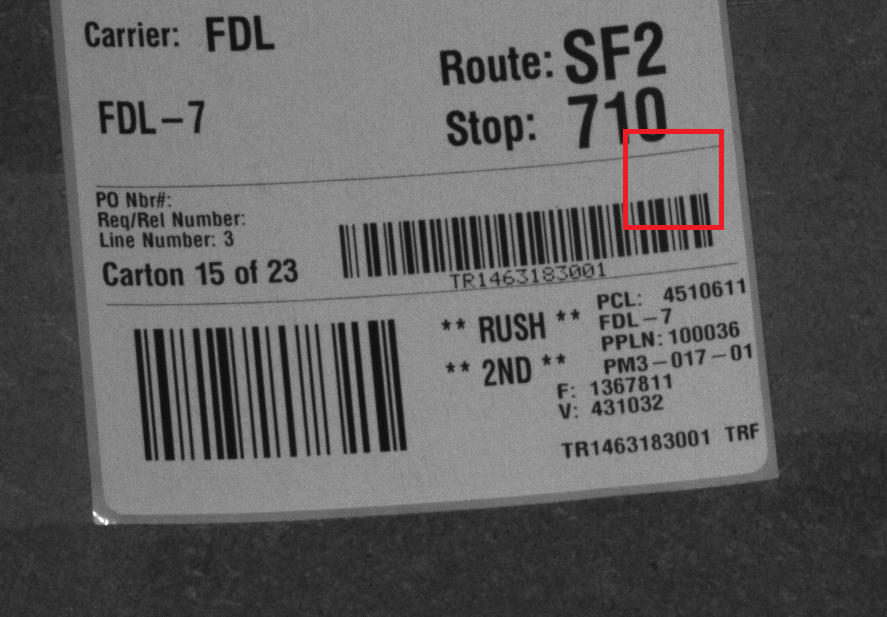
\includegraphics[scale=0.3]{evaluationGroundTruth}
	\caption{Image illustrates an example when the tile is too large}
	\label{evaluationGroundTruth}
\end{figure}

There are not really any good way to evaluate which tile size and how much overlap that is necessary. The size of the codes in the dataset varies and there are not many images which contains these thin 1D-codes. However by inspecting the result of some difficult images one can make a rather good assessment. 

If the tile size is more than 64x64 it will be too big and some of the 1D-codes will not be detected even if the tiles overlap each other. But there are also no reason to use too small tiles. If the tiles are too small the pattern which characterize the codes might get lost.

In table \ref{table:overlap} some tile sizes have been tried out with different down sampling. The values written in the table is how much overlap of the tiles which is necessary to achieve an acceptable result. The cells in the table which are empty are cases when it's not possible to get a good result. For example if the overlap is 2 the tiles will overlap half of there adjacent tiles. If the overlap is 3 the tiles will overlap 2/3 of there adjacent tiles. Overlap 1 means no overlap. 

\begin{table}[H]
\begin{center}
     \begin{tabular}{ | l | l | l | l | l | p{5cm} |}
     \hline
     tile size & no down sample & down sample 2 & down sample 3 & down sample 4 \\ \hline
   	 24x24 & 1 & 1-2 & 3 & 	\\ \hline
     32x32 & 1 & 2-3 &   & 	\\ \hline
     48x48 & 2 &     &   &  \\ \hline
     64x64 & 3 &     &   &	\\ \hline
     \end{tabular}
\end{center}
\caption{Necessary overlap of the tiles to calculate ground truth}
\label{table:overlap}
\end{table}

Figure \ref{evaluationGroundTruth2} shows an example for the case when the tile size is 24x24, no overlapping tiles and the image is down sampled with 2
\begin{figure}[H]
\centering
	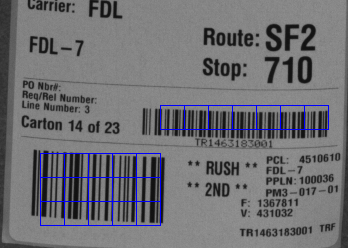
\includegraphics[scale=1]{evaluationGroundTruth2}
	\caption{Image illustrates an example for the case when the tile size is 24x24, no overlapping tiles and the image is down sampled with 2}
	\label{evaluationGroundTruth2}
\end{figure}

\section{Evaluation of features for AdaBoost}
\label{sec:Evaluation of features for AdaBoost}
Here is an evaluation of each feature that are used in the cascade presented in section \ref{sec:Code detection with AdaBoost}. The objective is to keep as many true tiles as possible in each step of the cascade and in the same time reduce the amount of date as much as possible. In this evaluation the objective has been to preserve at least 95\% of the true tiles in each step. Here different tile sizes and different amount of down sampling have been tried and best value of $\varphi$ has been calculated to preserve 95\% of the true tiles and as few false tiles as possible. Here only cases which gave a good result in the evaluation of the ground truth above are tested. 

\subsection{Standard deviation}
When using standard deviation the images have been preprocessed with Laplace filtering and no overlapping tiles. It has been trained on both 1D- and 2D-codes. 

\begin{table}[H]
\begin{center}
     \begin{tabular}{ | l | l | l | l | l |}
     \hline
     tile size & no down sample & down sample 2 & down sample 3 \\ \hline
   	 24x24 & 4 & 4 & 4 			\\ \hline
     32x32 & 4 & 4  & 			\\ \hline
     48x48 & 3 &     &  		\\ \hline
     64x64 & 3 &     &			\\ \hline
     \end{tabular}
\end{center}
\caption{Lowest value of $\varphi$ that keeps at least 95\% of the true tiles when using standard deviation}
\end{table}

\begin{table}[H]
\begin{center}
     \begin{tabular}{ | l | l | l | l | l |}
     \hline
     tile size & no down sample & down sample 2 & down sample 3 \\ \hline
   	 24x24 & 280 & 12.23 & 33.6 	\\ \hline
     32x32 & 96.27 & 163 & 			\\ \hline
     48x48 & 77    &     &  		\\ \hline
     64x64 & 69     &     &			\\ \hline
     \end{tabular}
\end{center}
\caption{The average number of false detection per image using standard deviation}
\end{table}

\subsection{Structure tensor}
When using structure tensor the images have been preprocessed with Laplace filtering and no overlapping tiles. It has been trained only on 1D-codes. 

\begin{table}[H]
\begin{center}
     \begin{tabular}{ | l | l | l | l | l |}
     \hline
     tile size & no down sample & down sample 2 & down sample 3 \\ \hline
   	 24x24 & 1.5-2 & 2.5 & bad result 	\\ \hline
     32x32 & 1 & 2  & 					\\ \hline
     48x48 & 1.5 &     &  				\\ \hline
     64x64 & 1 &     &					\\ \hline
     \end{tabular}
\end{center}
\caption{Lowest value of $\varphi$ that keeps at least 95\% of the true tiles when using structure tensor}
\end{table}

\begin{table}[H]
\begin{center}
     \begin{tabular}{ | l | l | l | l | l |}
     \hline
     tile size & no down sample & down sample 2 & down sample 3 \\ \hline
   	 24x24 & 226 & 121 & bad result 	\\ \hline
     32x32 & 92 & 228 & 				\\ \hline
     48x48 & 23    &     &  			\\ \hline
     64x64 & 28     &     &				\\ \hline
     \end{tabular}
\end{center}
\caption{The average number of false detection per image using structure tensor}
\end{table}

\subsection{Distance map}
The distance map is trained only with 1D-codes and without Laplace filtering.

\begin{table}[H]
\begin{center}
     \begin{tabular}{ | l | l | l | l | l |}
     \hline
     tile size & no down sample & down sample 2 & down sample 3 \\ \hline
   	 24x24 & 1 & 1.5 & 2 		\\ \hline
     32x32 & 1 & 1.5  & 		\\ \hline
     48x48 & 1 &     &  		\\ \hline
     64x64 & 1.2 &     &		\\ \hline
     \end{tabular}
\end{center}
\caption{Lowest value of $\varphi$ that keeps at least 95\% of the true tiles when using distance map}
\end{table}

\begin{table}[H]
\begin{center}
     \begin{tabular}{ | l | l | l | l | l |}
     \hline
     tile size & no down sample & down sample 2 & down sample 3 \\ \hline
   	 24x24 & 90 & 15 & 71 	    \\ \hline
     32x32 & 35 & 23 & 			\\ \hline
     48x48 & 45    &     &  	\\ \hline
     64x64 & 52     &     &		\\ \hline
     \end{tabular}
\end{center}
\caption{The average number of false detection per image using distance map}
\end{table}


\subsection{FAST corner detection}
The FAST corner detection feature is trained only with 2D-codes and without Laplace filtering. When down sampling with 3 the result seems to drop significantly, then it seems like it detects a lot of corners in the 1D-code.

\begin{table}[H]
\begin{center}
     \begin{tabular}{ | l | l | l | l | l |}
     \hline
     tile size & no down sample & down sample 2 & down sample 3 \\ \hline
   	 24x24 & 1.5 & 4 & 3 		\\ \hline
     32x32 & 3 & 4 & 			\\ \hline
     48x48 & 2.2 &     &  		\\ \hline
     64x64 & 3 &     &			\\ \hline
     \end{tabular}
\end{center}
\caption{Lowest value of $\varphi$ that keeps at least 95\% of the true tiles when using FAST corner detection}
\end{table}

\begin{table}[H]
\begin{center}
     \begin{tabular}{ | l | l | l | l | l |}
     \hline
     tile size & no down sample & down sample 2 & down sample 3 \\ \hline
   	 24x24 & 75 & 17 & 138		\\ \hline
     32x32 & 59 & 21 & 			\\ \hline
     48x48 & 80    &     &  	\\ \hline
     64x64 & 44     &     &		\\ \hline
     \end{tabular}
\end{center}
\caption{The average number of false detection per image using FAST corner detection}
\end{table}

\subsection{Local binary pattern}
\label{subsec:Local binary pattern}
The LBP feature is trained only with 2D-codes and without Laplace filtering. The evaluation was in this case done together with the cascade. The reason for this is that it takes too long to test this features for all data. When using the cascade the data is reduced a lot before the step where the LBP is used. Also the training was done with 50 weak classifiers instead of 100.

\begin{table}[H]
\begin{center}
     \begin{tabular}{ | l | l | l | l | l |}
     \hline
     tile size & no down sample & down sample 2 & down sample 3 \\ \hline
   	 24x24 &  & 3 & 		\\ \hline
     32x32 &  & 2 & 			\\ \hline
     48x48 & 2 &     &  		\\ \hline
     64x64 & 2 &     &			\\ \hline
     \end{tabular}
\end{center}
\caption{Lowest value of $\varphi$ that keeps at least 98\% of the true tiles when using LBP}
\end{table}


\section{Result for AdaBoost classifiers in a cascade}
\label{sec:Result for AdaBoost classifiers in a cascade}
Here are some conclusions that can be drawn from the evaluation of the features before evaluating the cascade.

\begin{itemize}
\item There is no reason to use tiles with sizes 24x24 and 32x32 without down sampling with 2, since all feature seems to work in this case.

\item To down sample with more than 2 seems to give really bad results with structure tensor.

\item The cascade will be a lot faster with down sampling with 2 and tile sizes 24x24 and 32x32. This is because the amount of false tiles when using standard deviation are very low.
\end{itemize}

From these conclusions the evaluation of the cascade will be done for four different cases regarding the tile size, the down sampling and the overlap of the tiles. Also the cascades has been evaluated for the two different variants which was described in section \ref{sec:Code detection with AdaBoost}. Here is the result from cascade 1.

\begin{table}[H]
\begin{center}
     \begin{tabular}{ | p{3cm} | l | p{3cm} | p{2cm}|}
     \hline
      	& time per image & true detections & false tiles \newline per image \\ \hline
   	 tile size 24x24 \newline down sampling 2 \newline overlap 1 
   	 & 75 ms & 1D: 98\% \newline 2D: 95\% & 1D: 0.7 \newline 2D: 0.14 				\\ \hline
     tile size 32x32 \newline down sampling 2 \newline overlap 2 
     & 190 ms & 1D: 98\% \newline 2D: 93\% & 1D: 0.26 \newline 2D: 0				\\ \hline
     tile size 48x48 \newline down sampling 1 \newline overlap 2 
     & 420 ms & 1D: 96\% \newline 2D: 94.5\% & 1D: 0.3 \newline 2D: 0.097
     \\ \hline
     tile size 64x64 \newline down sampling 1 \newline overlap 3 
     & 631 ms & 1D: 96\% \newline 2D: 93\% & 1D: 0.35 \newline 2D: 0.93		 \\ \hline
     \end{tabular}
\end{center}
\caption{Result from evaluation of cascade 1}
\label{table:ResultAdaBoost1}
\end{table}

Here is the evaluation of cascade 2.
\begin{table}[H]
\begin{center}
     \begin{tabular}{ | p{3cm} | l | p{3cm} | p{2cm}|}
     \hline
      	& time per image & true detections & false tiles \newline per image \\ \hline
   	 tile size 24x24 \newline down sampling 2 \newline overlap 1 
   	 & 74 ms & 1D: 96\% \newline 2D: 95\% & 1D: 0.5 \newline 2D: 0.12 				\\ \hline
     tile size 32x32 \newline down sampling 2 \newline overlap 2 
     & 210 ms & 1D: 97\% \newline 2D: 94\% & 1D: 0.18 \newline 2D: 0				\\ \hline
     tile size 48x48 \newline down sampling 1 \newline overlap 2 
     & 390 ms & 1D: 96\% \newline 2D: 94.5\% & 1D: 0.02 \newline 2D: 0.097
     \\ \hline
     tile size 64x64 \newline down sampling 1 \newline overlap 3 
     & 630 ms & 1D: 96\% \newline 2D: 93\% & 1D: 0.18 \newline 2D: 0		 \\ \hline
     \end{tabular}
\end{center}
\caption{Result from evaluation of cascade 2}
\label{table:ResultAdaBoost2}
\end{table}

Bellow is the result from the first two tests of cascade 1 (first two row in table \ref{table:ResultAdaBoost1}).
\begin{figure}[H]
\centering
	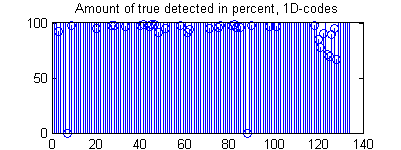
\includegraphics {codesBoost24true1D}
	\caption{Amount of true detections for 1D-codes from evaluation of cascade using tile size 24x24, down sampling 2, and no overlap}
	\label{codeBoost24true1D}
\end{figure}

\begin{figure}[H]
\centering
	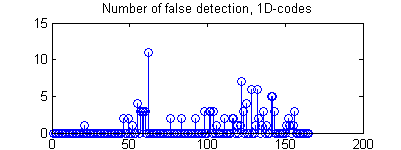
\includegraphics {codesBoost24false1D}
	\caption{Number of false detections for 1D-codes from evaluation of cascade using tile size 24x24, down sampling 2, and no overlap}
	\label{codeBoost24false1D}
\end{figure}

\begin{figure}[H]
\centering
	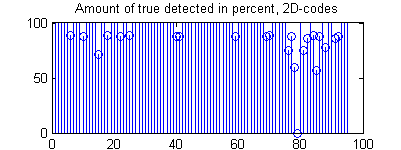
\includegraphics {codesBoost24true2D}
	\caption{Amount of true detections for 2D-codes from evaluation of cascade using tile size 24x24, down sampling 2, and no overlap}
	\label{codeBoost24true2D}
\end{figure}

\begin{figure}[H]
\centering
	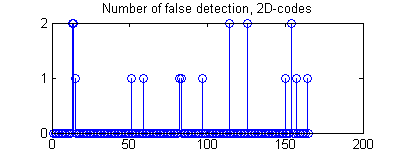
\includegraphics {codesBoost24false2D}
	\caption{Number of false detections for 2D-codes from evaluation of cascade using tile size 24x24, down sampling 2, and no overlap}
	\label{codeBoost24false2D}
\end{figure}

\begin{figure}[H]
\centering
	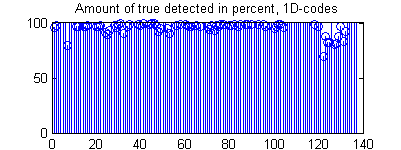
\includegraphics {codesBoost32true1D}
	\caption{Amount of true detections for 1D-codes from evaluation of cascade using tile size 32x32, down sampling 2, and no overlap}
	\label{codeBoost32true1D}
\end{figure}

\begin{figure}[H]
\centering
	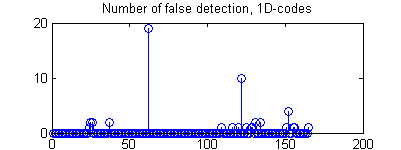
\includegraphics {codesBoost32false1D}
	\caption{Number of false detections for 1D-codes from evaluation of cascade using tile size 32x32, down sampling 2, and no overlap}
	\label{codeBoost32false1D}
\end{figure}

\begin{figure}[H]
\centering
	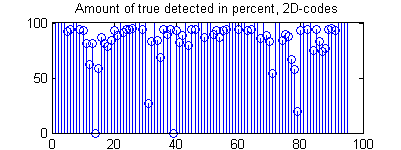
\includegraphics {codesBoost32true2D}
	\caption{Amount of true detections for 2D-codes from evaluation of cascade using tile size 32x32, down sampling 2, and no overlap}
	\label{codeBoost32true2D}
\end{figure}

\begin{figure}[H]
\centering
	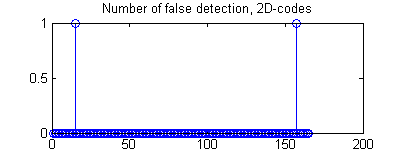
\includegraphics {codesBoost32false2D}
	\caption{Number of false detections for 2D-codes from evaluation of cascade using tile size 32x32, down sampling 2, and no overlap}
	\label{codeBoost32false2D}
\end{figure}

\begin{figure}[H]
\centering
	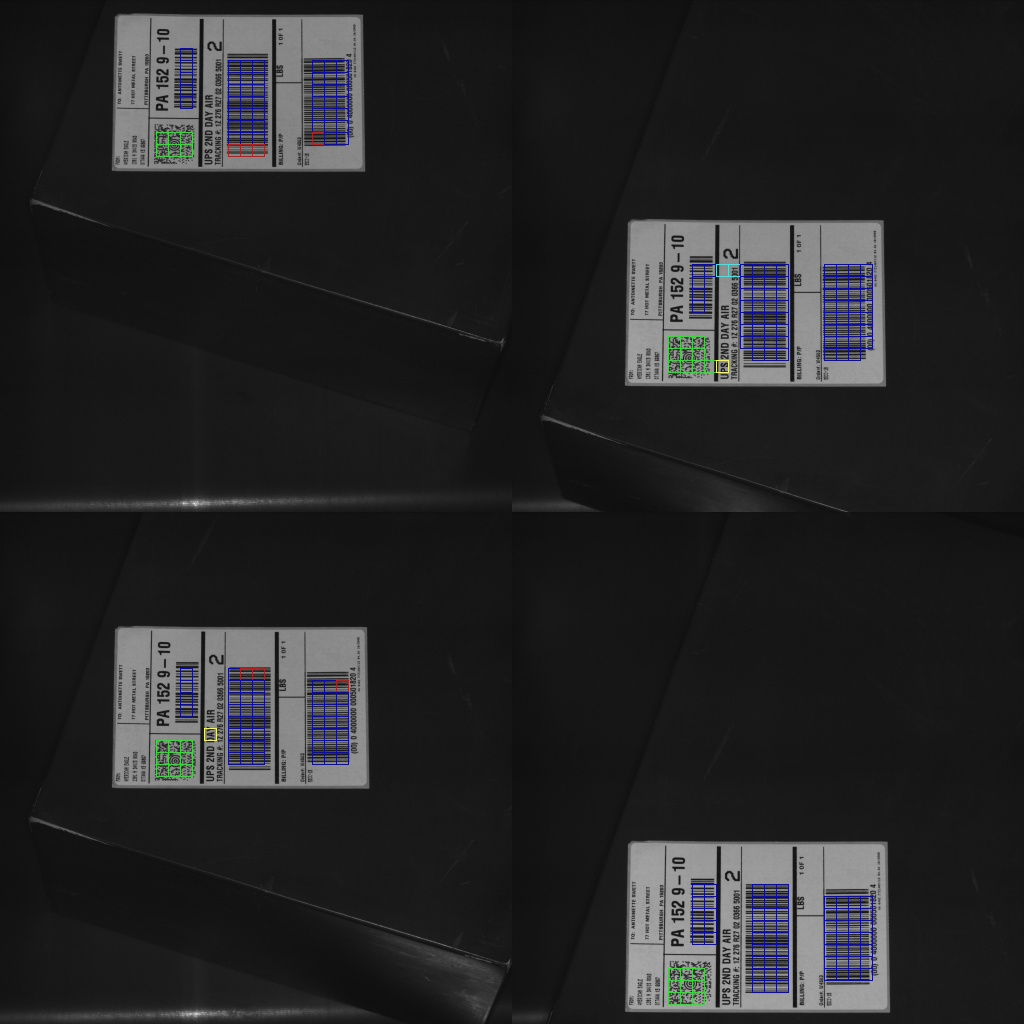
\includegraphics[scale=0.25]{Result24x24}
	\caption{Result from evaluation of cascade using tile size 32x32, down sampling 2, and overlap 2}
	\label{Result24x24}
\end{figure}

\section{Evaluation of Random forest}
\label{sec:Evaluation of Random forest}
When the system is trained with Random forest all features except standard deviation is used in the same classifier, as was explained in section \ref{sec:Code detection with Random forest}. For that reason the features are not evaluated individually like it was for AdaBoost in section \ref{sec:Evaluation of features for AdaBoost}.
  
When using Random forest it is possible to control the amount of true detections by having a threshold for the number of votes in the strong classifier. For example 1D-codes might belong to class 1 and have the threshold 10\%. This means that at least 10\% of all trees need to predict class 1 to make it the final prediction. Table \ref{table:thresholdRandomForest} shows this threshold for 1D- and 2D-codes for the same cases as was evaluated in section \ref{sec:Result for AdaBoost classifiers in a cascade}, for different number of trees. Table \ref{tabel:trueRF} shows the amount of true detections in percent, table \ref{tabel:falseRF} shows the number of false detection and table \ref{tabel:timeRF} shows the average time per image. 

\begin{table}[H]
\begin{center}
     \begin{tabular}{ | p{3cm} | p{2cm} | p{2cm} | p{2cm}|}
     \hline
      	& 50 trees & 100 trees & 500 trees \\ \hline
   	 tile size 24x24 \newline down sampling 2 \newline overlap 1 &
   1D: 75\% \newline 2D: 24\% & 1D: 60\% \newline 2D: 24\% & 1D: 60\% \newline 2D: 24\%  				\\ \hline
     tile size 32x32 \newline down sampling 2 \newline overlap 2 &
    1D: 70\% \newline 2D: 22\% & 1D: 60\% \newline 2D: 24\%  & 1D: 70\% \newline 2D: 		24 	 \\ \hline
     tile size 48x48 \newline down sampling 1 \newline overlap 2 
     & 1D: \newline 2D: & 1D: \newline 2D:  & 1D:\newline 2D: 
     \\ \hline
     tile size 64x64 \newline down sampling 1 \newline overlap 3 
     & 1D: \newline 2D: & 1D:  \newline 2D:  & 1D:  \newline 2D: 		 \\ \hline
     \end{tabular}
\end{center}
\caption{Threshold for the amount of votes for 1D- and 2D-codes respectively}
\label{table:thresholdRandomForest}
\end{table}

\begin{table}[H]
\begin{center}
     \begin{tabular}{ | p{3cm} | p{2cm} | p{2cm} | p{2cm}|}
     \hline
      	& 50 trees & 100 trees & 500 trees \\ \hline
   	 tile size 24x24 \newline down sampling 2 \newline overlap 1 &
   	1D: 96\%  \newline 2D: 97.7\% & 1D: 99.8\%  \newline 2D: 96.7\% & 1D: 99.8\%  \newline 2D: 97.8\%				\\ \hline
     tile size 32x32 \newline down sampling 2 \newline overlap 2 &
   1D: 97.4\% \newline 2D: 96.6\% &  1D: 99.7\%  \newline 2D: 97.8\% & 1D: 97.6\%  \newline 2D: 98.4\%			\\ \hline
     tile size 48x48 \newline down sampling 1 \newline overlap 2 &
   1D:  \newline 2D:  &  1D:  \newline 2D:  & 1D: \newline 2D:
     \\ \hline
     tile size 64x64 \newline down sampling 1 \newline overlap 3 
     & 1D: \newline 2D: & 1D: \newline 2D:  & 1D: \newline 2D: 		 \\ \hline
     \end{tabular}
\end{center}
\caption{Amount of true detections for 1D- and 2D-codes respectively}
\label{tabel:trueRF}
\end{table}

\begin{table}[H]
\begin{center}
     \begin{tabular}{ | p{3cm} | p{2cm} | p{2cm} | p{2cm}|}
     \hline
      	& 50 trees & 100 trees & 500 trees \\ \hline
   	 tile size 24x24 \newline down sampling 2 \newline overlap 1 &
   	1D: 0.24  \newline 2D: 0.50 & 1D: 3.24 \newline 2D: 0.13 &  1D: 1.63 \newline 2D: 0.28  	\\ \hline
     tile size 32x32 \newline down sampling 2 \newline overlap 2 &
    1D: 0.15 \newline 2D: 0 & 1D: 0.9 \newline 2D: 0 & 1D: 0.06  \newline 2D: 0  				\\ \hline
     tile size 48x48 \newline down sampling 1 \newline overlap 2 
     & 1D: \newline 2D: & 1D: \newline 2D: & 1D: \newline 2D: 
     \\ \hline
     tile size 64x64 \newline down sampling 1 \newline overlap 3 
     & 1D: \newline 2D: & 1D: \newline 2D:  & 1D: \newline 2D: 		 \\ \hline
     \end{tabular}
\end{center}
\caption{Number of false detections for 1D- and 2D-codes respectively}
\label{tabel:falseRF}
\end{table}

\begin{table}[H]
\begin{center}
     \begin{tabular}{ | p{3cm} | p{2cm} | p{2cm} | p{2cm}|}
     \hline
      	& 50 trees & 100 trees & 500 trees \\ \hline
   	 tile size 24x24 \newline down sampling 2 \newline overlap 1 
   	 & 84 ms & 86 ms  & 109 ms 				\\ \hline
     tile size 32x32 \newline down sampling 2 \newline overlap 2 
     & 192 ms & 197 ms & 257 ms 				\\ \hline
     tile size 48x48 \newline down sampling 1 \newline overlap 2 
     &     &  &  \\ \hline
     tile size 64x64 \newline down sampling 1 \newline overlap 3 
     &  &  &	 \\ \hline
     \end{tabular}
\end{center}
\caption{Average time per image}
\label{tabel:timeRF}
\end{table}

\section{Conclusions}
\label{sec:Conclusions}
The two variants of the cascade gave rather similar results. Both the structure tensor and the FAST corner detection are rather good at distinguish between 1D- and 2D-codes.

The first two cases (the two first rows in table \ref{table:ResultAdaBoost1} and table \ref{table:ResultAdaBoost2}) gives overall better result, especially regarding the speed. Which one of them that is best depend of what is required of the system, regarding speed and accuracy.

One alternative is to omit the distance map feature in the cascade and only use standard deviation and structure tensor for detection of 1D-codes. The result is still rather good, the amount of true detections is even higher but the amount of false tiles will increase.

The amount of true tiles detected can in some cases seem a bit weak, especially for 2D-codes. In graph \ref{codeBoost24true2D} one can see that in one image there are no detections at all. This is the case when the codes are at the border of the image and only a small part are inside. Since in this case only a few tiles will cover the codes there is a big chance that these will be lost in the post-processing. The alternative is to reduce the amount of post-processing but this will instead lead to more false tiles.  

For code detection some different features have been used, some of them are more computational then others. This makes it less suitable for random forest.  
% Local Variables:
% TeX-master: "main.tex"
% End:
